\section{Installing CSipSimple}

CSipSimple is a program for Android devices that allows for making
encrypted calls. Naturally the calling software isn't enough on its own
and we need a communication network to enable us to make calls.

\subsection{Introducing The OSTN Network}

If you already know about OSTN and have an account, you can skip this
section.

OSTN (Open \{Secure, Source, Standards\} Telephony Network -
\href{https://guardianproject.info/wiki/OSTN}{https://guardianproject.info/wiki/OSTN})
is an attempt to define a standard Voice over IP (VoIP) setup using the
Session Initiation Protocol (SIP) that enables end-to-end encrypted
calls. Similar to e-mail, SIP allows people to choose their service
provider while still being able to call each other even if they are not
using the same provider. Yet, not all SIP providers offer OSTN and both
providers have to support OSTN for the call to be secure. Once a
connection between two people is established, the audio data is
exchanged directly between the two parties. Data is encrypted according
to the Secure Real-time Transport Protocol (SRTP).

A majority of encrypting VoIP applications currently use Session
Description Protocol Security Descriptions for Media Streams (SDES) with
hop-by-hop Transport Layer Security (TLS) to exchange secret master keys
for SRTP. This method is not end-to-end secure as the SRTP keys are
visible in plaintext to any SIP proxy or provider involved in the call.

ZRTP is a cryptographic key-agreement protocol to negotiate the keys for
encryption between two parties. ZRTP end points use the media stream
rather than the signaling stream to establish the SRTP encryption keys.
Since the media stream is a direct connection between the calling
parties, there is no way for the SIP providers or proxies to intercept
the SRTP keys. ZRTP provides a useful reassurance to end-users that they
have a secure line. By reading and comparing a word pair, users can be
certain that the key exchange has completed.

Open Secure Telephony (https://ostel.me/) is a testbed for OSTN that
worked well at the time of writing this book. At
https://ostel.me/users/sign\_up you can sign up and create an account.
You can also check the OSTN page listed above for other providers.

\subsection{CSipSimple}

CSipSimple is a free and open source client for Android that works well
with OSTN. You can find it at
\href{https://market.android.com/details?id=com.csipsimple}{https://market.android.com/details?id=com.csipsimple}

To use CSipSimple with ostel.me, select OSTN in the generic wizards when
creating an account and enter username, password and server as provided
after signing up at
\href{https://ostel.me/users/sign\_up}{https://ostel.me/users/sign\_up}

Once you call another party with CSipSimple you see a yellow bar with
ZRTP and the verification word pair. You now have established a secure
voice connection that cannot be intercepted. Still, you should be aware
that your phone or the phone of the other party could be set up to
record the conversation.

Basic steps:

\begin{enumerate}[1.]
\item
  Install CSipSimple from Google Play store or other trusted source
\item
  Start it up and choose if you want to make SIP calls via data
  connection or only WiFi
\item
  Configure your account
\end{enumerate}
To use CSipSimple with ostel.me, select OSTN in the Generic Wizards
section when creating an account. You can toggle off the ``United
States'' providers by clicking on ``United States''. Now select
\emph{OSTN}:

\begin{figure}[htbp]
\centering
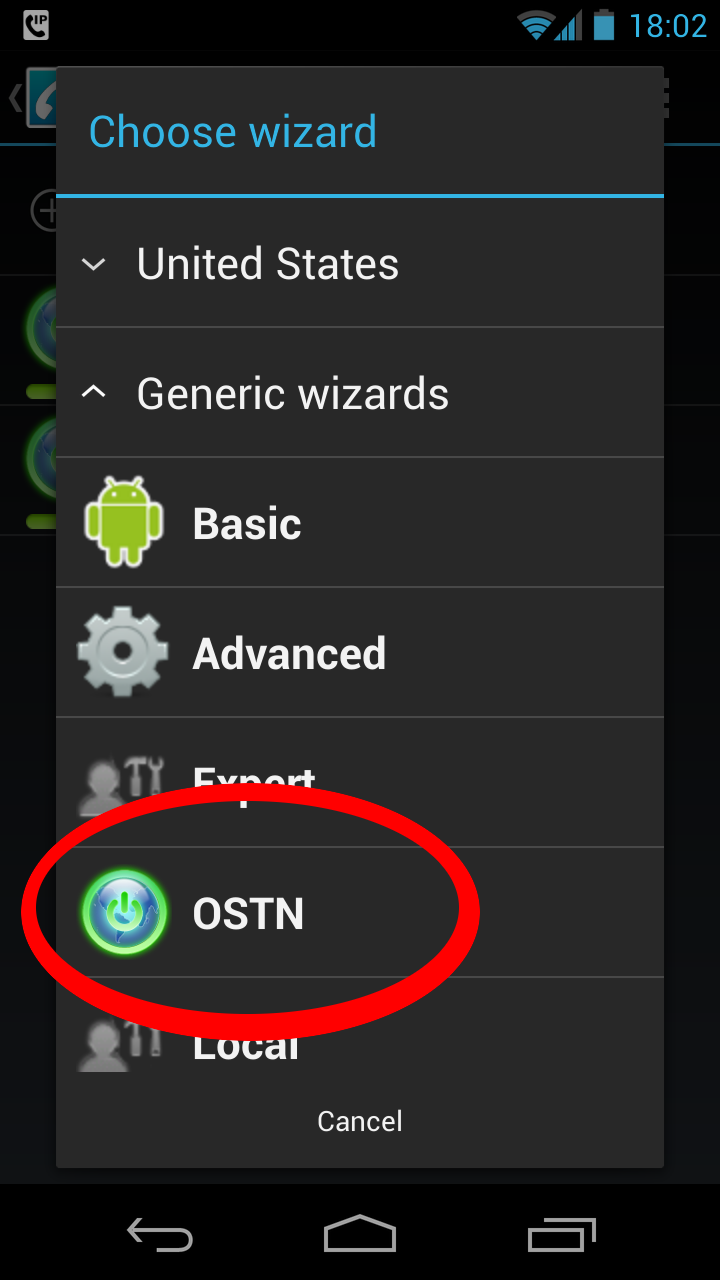
\includegraphics{ostn_1.png}
\caption{OSTN}
\end{figure}

Now you can enter your username (number), password and server (ostel.me)
as provided after signing up at
\href{https://ostel.me/users/sign\_up}{https://ostel.me/users/sign\_up}.

\begin{figure}[htbp]
\centering
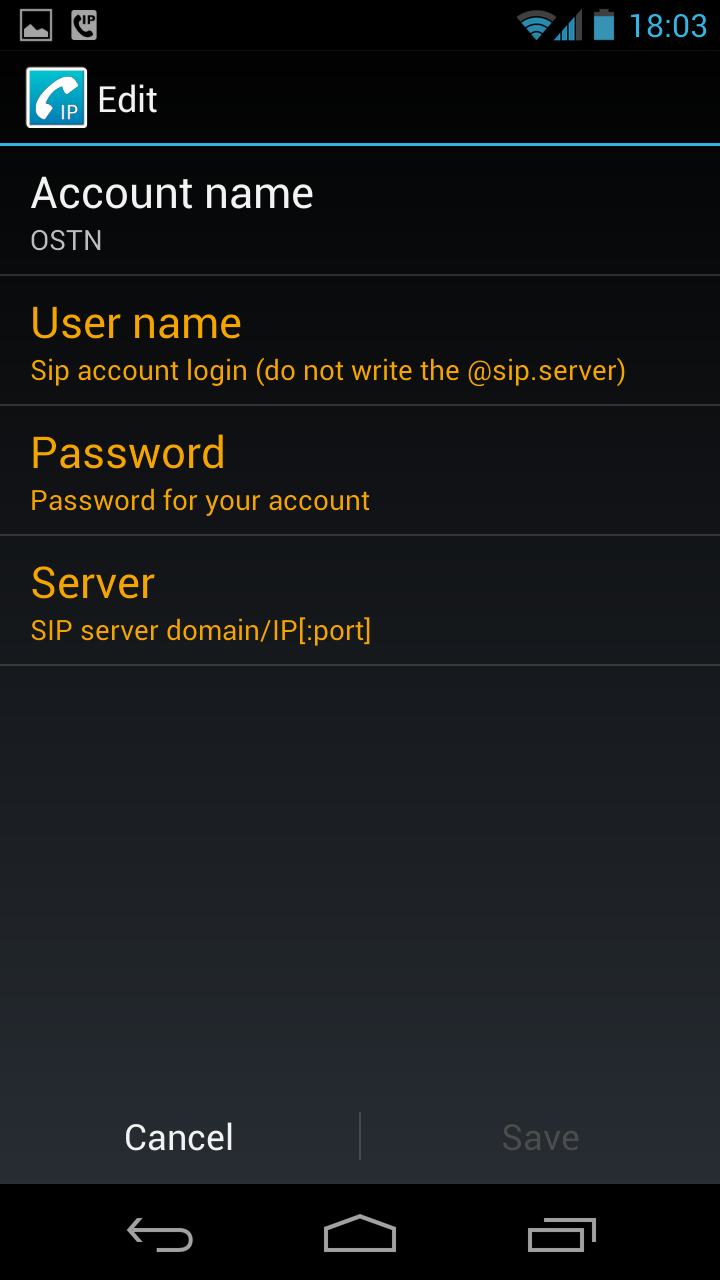
\includegraphics{ostn_2.png}
\caption{OSTN}
\end{figure}

Now you can make a call. The first time you connect to someone with ZRTP
you have to verify that the key exchange was successful. In the example
below the confirmation word is ``cieh'', you can already talk to the
other party and make sure you both see the same word. Once done, press
ok.

\begin{figure}[htbp]
\centering
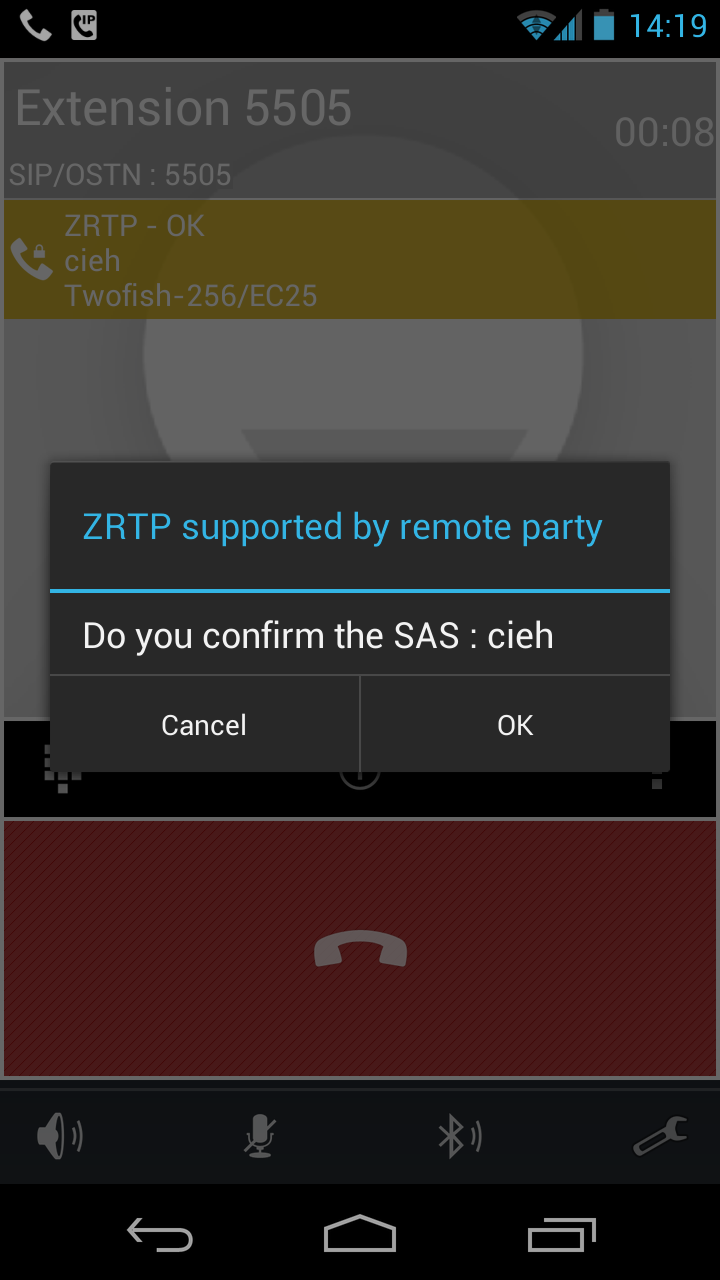
\includegraphics{ostn_3.png}
\caption{OSTN}
\end{figure}

You now have established a secure voice connection that cannot be
intercepted. Beware that your or the phone of the other party could be
recording your conversation.
